\section{Input-Mapper Programm}
Das Input-Mapper Programm dient mit einer grafischen Oberfläche zu Steuerung, Konfiguration und Kontrolle der angeschlossenen Module. Es ist der Hauptbestandteil der Kommunikation zwischen dem Hauptmodul und dem verbundenen Computer. Das Programm wurde entwickelt, um den Tasten des Keypads und den Funktionen zukünftiger Module bestimmte Funktionen zuzuweisen, wie z.B. das Ausführen von Tastenkombinationen auf dem Computer. Die derzeitige Hauptfunktionalität besteht darin, das Keypad mit dem 4x4 Tastenraster zu individualisieren. Das Programm ist in Python geschrieben und verwendet die grafische Benutzeroberfläche der Bibliothek \glqq customtkinter\grqq.


\begin{figure}[H]
	\centering    
	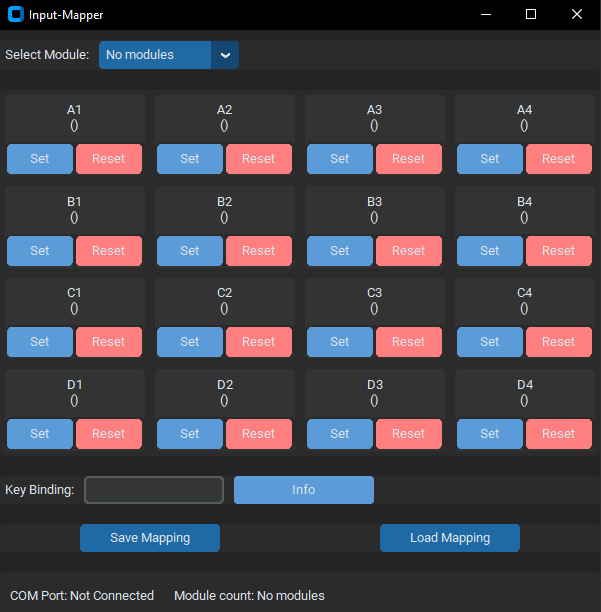
\includegraphics[width=.8\textwidth]{Bilder/mapper.png}
	\caption{Benutzeroberfläche des Inputmapper-Programms}
	\label{Mapper_ui}
\end{figure}
Abbildung \ref{Mapper_ui} zeigt die grafische Benutzeroberfläche des Input-Mapper Programms. Es bietet eine Auswahl der verbundenen Module und die Möglichkeit, die Tasten dieses Moduls nach Belieben zu individualisieren. In das Eingabefenster \glqq Key Binding:\grqq{} wird die gewünschte Tastenkombination eingetragen und danach bei der einer Taste auf \glqq Set\grqq{} gedrückt. Ab diesem Zeitpunkt wird diese Taste beim Drücken, die hinterlegte Kombination ausführen oder Zeichenkette ausgeben. Das Infofenster bietet eine beispielhafte Übersicht einiger Tastenbelegungen. \glqq Save Mapping\grqq{} und \glqq Load Mapping\grqq{} werden benutzt, um Konfigurationen zu speichern oder zu laden. Zuletzt wird dem Benutzer eine Übersicht über den verwendeten COM-Port und die Anzahl aller verbundenen Module geboten.

\subsection{Hauptfunktionen}
\begin{enumerate}
    \item \textbf{Hardware-Erkennung:} Das Programm durchsucht alle verfügbaren COM-Ports des angeschlossenen Computers und vergleicht deren Inputs mit der Initialisierungsnachricht. An dem Port, an dem eine Nachricht \glqq INIT\grqq{} anliegt, wird als Kontroller-Port für das modulare Eingabesystem erkannt.
    \item \textbf{Serielle-Kommunikation:} Über den COM-Port werden die Daten des Kontrollers (Modulliste oder gedrückte Taste des Moduls X) seriell übertragen und vom Programm ausgelesen. In der Funktion \glqq read\_from\_com\_port()\grqq{} werden kontinuierlich die verschiedenen möglichen Nachrichten geprüft und je nach Muster und Inhalt des Datenstroms verschiedene Funktionen im Programm aufgerufen.
    \item \textbf{Input-Mapping:} Der Benutzer bekommt die Möglichkeit, den Tasten des 4x4 Keypads individuelle Tastenkombinationen zuzuweisen. Dabei werden zusätzlich Normalisierungen vorgenommen, wie z.B. die Eingabe von \glqq ctrl\grqq{} in \glqq Control\grqq{} für eine bessere Lesbarkeit und Eingabefehler Minimierung.
    \item \textbf{Speichern und Laden:} Die Tastenzuordnungen können in einer JSON-Datei gespeichert und später wieder geladen werden. Diese Funktionen ermöglichen es dem Benutzer, bereits erstellte Konfigurationen auch zukünftig zu laden und zu verändern.
    \item \textbf{Modulverwaltung:} Das Programm erkennt automatisch verbundene Module und entfernt diese auch, sobald die Verbindung getrennt wurde. Dementsprechend wird das Dropdown-Menü zur Modulauswahl dynamisch angepasst.
    \newpage
    \item \textbf{GUI:}
        \begin{itemize}
            \item \textbf{Tastendarstellung:} Bei dem Keypad Modul wird jede Taste des 4x4 Rasters mit der aktuellen Belegung dargestellt.
            \item \textbf{Steuerelemente:} Es sind Knöpfe zum Setzen und Zurücksetzen von Tastenbelegungen, sowie zum Speichern und Laden von Konfigurationen vorhanden.
            \item \textbf{Kontrollelemente:} Das Programm bietet eine Übersicht der Anzahl an angeschlossenen Modulen und den COM-Port, über den die Nachrichten vom Kontroller-Modul übertragen werden.
            \item \textbf{Informationsfenster:} Der Benutzer kann ein Informationsfenster öffnen, in dem eine Vielzahl von Beispielbelegungen vorgegeben sind.
        \end{itemize}
\end{enumerate}

\begin{figure}[H]
	\centering    
	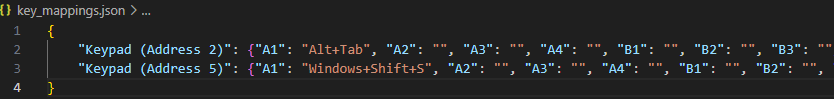
\includegraphics[width=1\textwidth]{Bilder/Save file.png}
	\caption{JSON-Datei zum Speichern und Laden von Konfigurationen}
	\label{Mapper_savefile}
\end{figure}
Abbildung \ref{Mapper_savefile} zeigt das Format, in welchem die Tastenbelegungen gespeichert werden. Wobei der Name des Moduls die ID oder auch \glqq Schlüssel\grqq{} zum eindeutigen Identifizieren ist. Zu dieser ID gehört dann eine Liste von Tasten und deren Zuweisung. Wobei bei der Taste \glqq A1\grqq{} das \glqq A\grqq{} für die Reihe der Taste und die \glqq 1\grqq{} für die Zeile der Taste steht.
\newpage
\begin{figure}[H]
	\centering    
	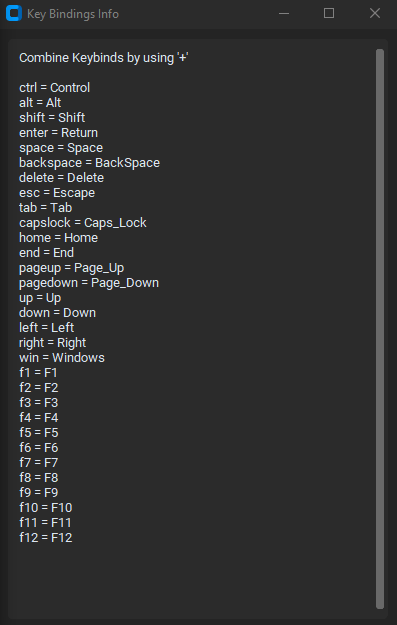
\includegraphics[width=.6\textwidth]{Bilder/Info_window.png}
	\caption{Infofenster mit beispielhaften Belegungen}
	\label{Mapper_info_window}
\end{figure}
Abbildung \ref{Mapper_info_window} zeigt das geöffnete Infofenster, in dem der Benutzer eine Vielzahl von beispielhaften Tastenkombinationen vorgegeben bekommt.